\chapter[Incertezas em SDM]{Incertezas em Modelagem de Distribuição de Espécies}

\begin{objetivos}
	Ao final desta unidade, o estudante deverá compreender as principais fontes de incerteza em SDM; diferenciar incerteza associada aos dados, algoritmos, cenários climáticos, extrapolação e escala espacial; quantificar incerteza algorítmica a partir de múltiplos modelos; avaliar incerteza entre cenários SSP; integrar incerteza de extrapolação ambiental; produzir mapas de incerteza para \textit{Dinizia excelsa}; e interpretar resultados de SDM de forma crítica, transparente e reprodutível.
\end{objetivos}

\section{Introdução}

Modelos de distribuição de espécies não produzem verdades absolutas sobre a distribuição das espécies. Eles produzem estimativas condicionadas aos dados de ocorrência, às variáveis ambientais, à área acessível, ao algoritmo, à parametrização, ao período climático e ao cenário de projeção. Portanto, toda aplicação robusta de SDM deve explicitar e quantificar incertezas \parencite{guisan2017habitat,franklin2023,zurell2020benchmarking,yates2018transferability}.

No caso de \textit{Dinizia excelsa}, as incertezas são particularmente importantes porque estamos trabalhando com uma espécie arbórea amazônica de grande porte, registros de ocorrência potencialmente enviesados, modelos climáticos, projeções futuras, reconstruções paleoclimáticas e extrapolação temporal.

\begin{conceito}[title={\faBook\quad Incerteza em SDM}]
	Incerteza é a variação ou limitação associada às estimativas do modelo. Em SDM, ela pode surgir dos dados de ocorrência, das variáveis ambientais, dos algoritmos, dos cenários climáticos, da extrapolação e da escala espacial.
\end{conceito}

\section{Fontes principais de incerteza}

Nesta unidade, organizamos as incertezas em cinco componentes principais:

\begin{itemize}
	\item incerteza dos dados de ocorrência;
	\item incerteza algorítmica;
	\item incerteza entre cenários climáticos;
	\item incerteza por extrapolação ambiental;
	\item incerteza espacial integrada.
\end{itemize}

\begin{atencao}[title={\faExclamationTriangle\quad Incerteza não é erro descartável}]
	Incerteza não deve ser escondida. Ela é parte fundamental da interpretação científica e ajuda a identificar onde as conclusões são robustas e onde devem ser tratadas com cautela.
\end{atencao}

\section{Incerteza algorítmica}

A incerteza algorítmica representa a divergência entre modelos ajustados com diferentes algoritmos. Nesta apostila, ela pode ser estimada pelo desvio-padrão das predições de GLM, GAM, Random Forest, BRT e Maxent.

\rscriptfile{scripts/unidade16/01_estrutura_pastas.R}

\rscriptfile{scripts/unidade16/02_incerteza_algoritmica_atual.R}

\begin{figure}[H]
	\centering
	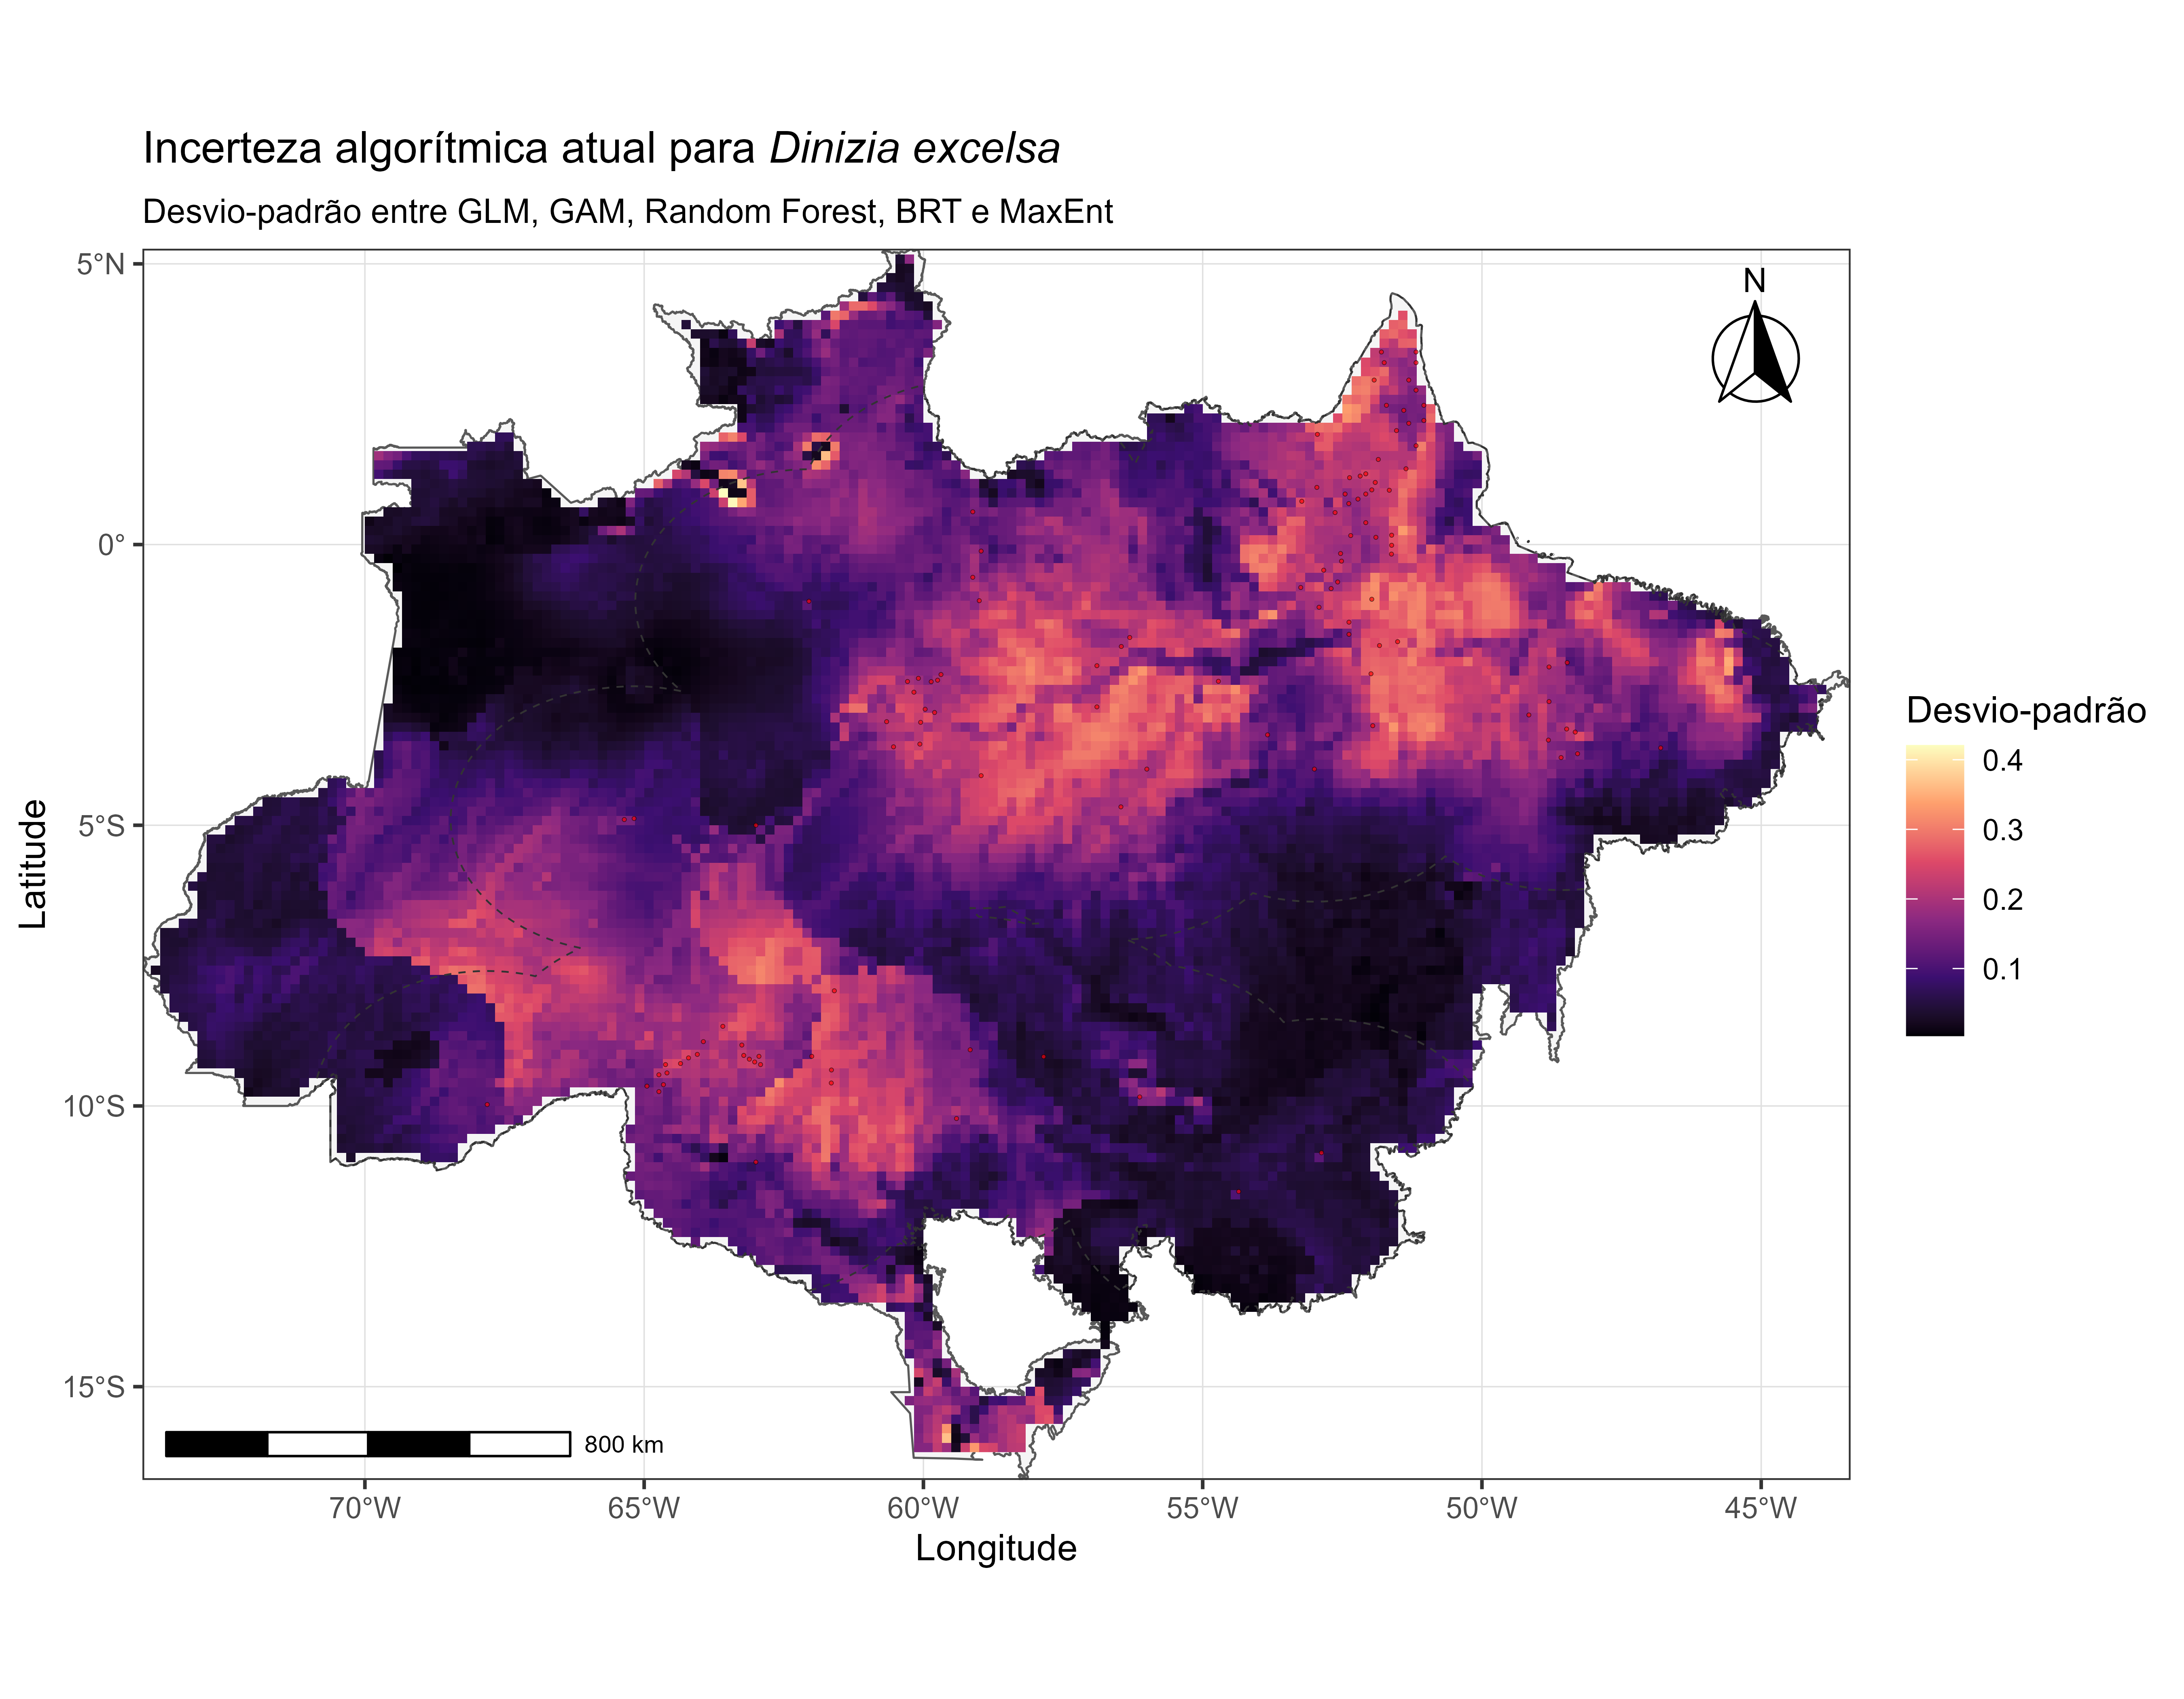
\includegraphics[width=0.88\textwidth]{figuras/unidade16/unidade16_incerteza_algoritmica_atual.png}
	\caption{Incerteza algorítmica atual para \textit{Dinizia excelsa}, estimada pelo desvio-padrão das predições entre GLM, GAM, Random Forest, BRT e Maxent.}
	\label{fig:unidade16_incerteza_algoritmica}
\end{figure}

\section{Incerteza entre cenários futuros}

A incerteza entre cenários representa a variação nas projeções futuras associada às diferentes trajetórias SSP. Nesta unidade, comparamos os ensembles futuros sob SSP126, SSP245, SSP370 e SSP585.

\rscriptfile{scripts/unidade16/03_incerteza_cenarios_futuros.R}

\begin{figure}[H]
	\centering
	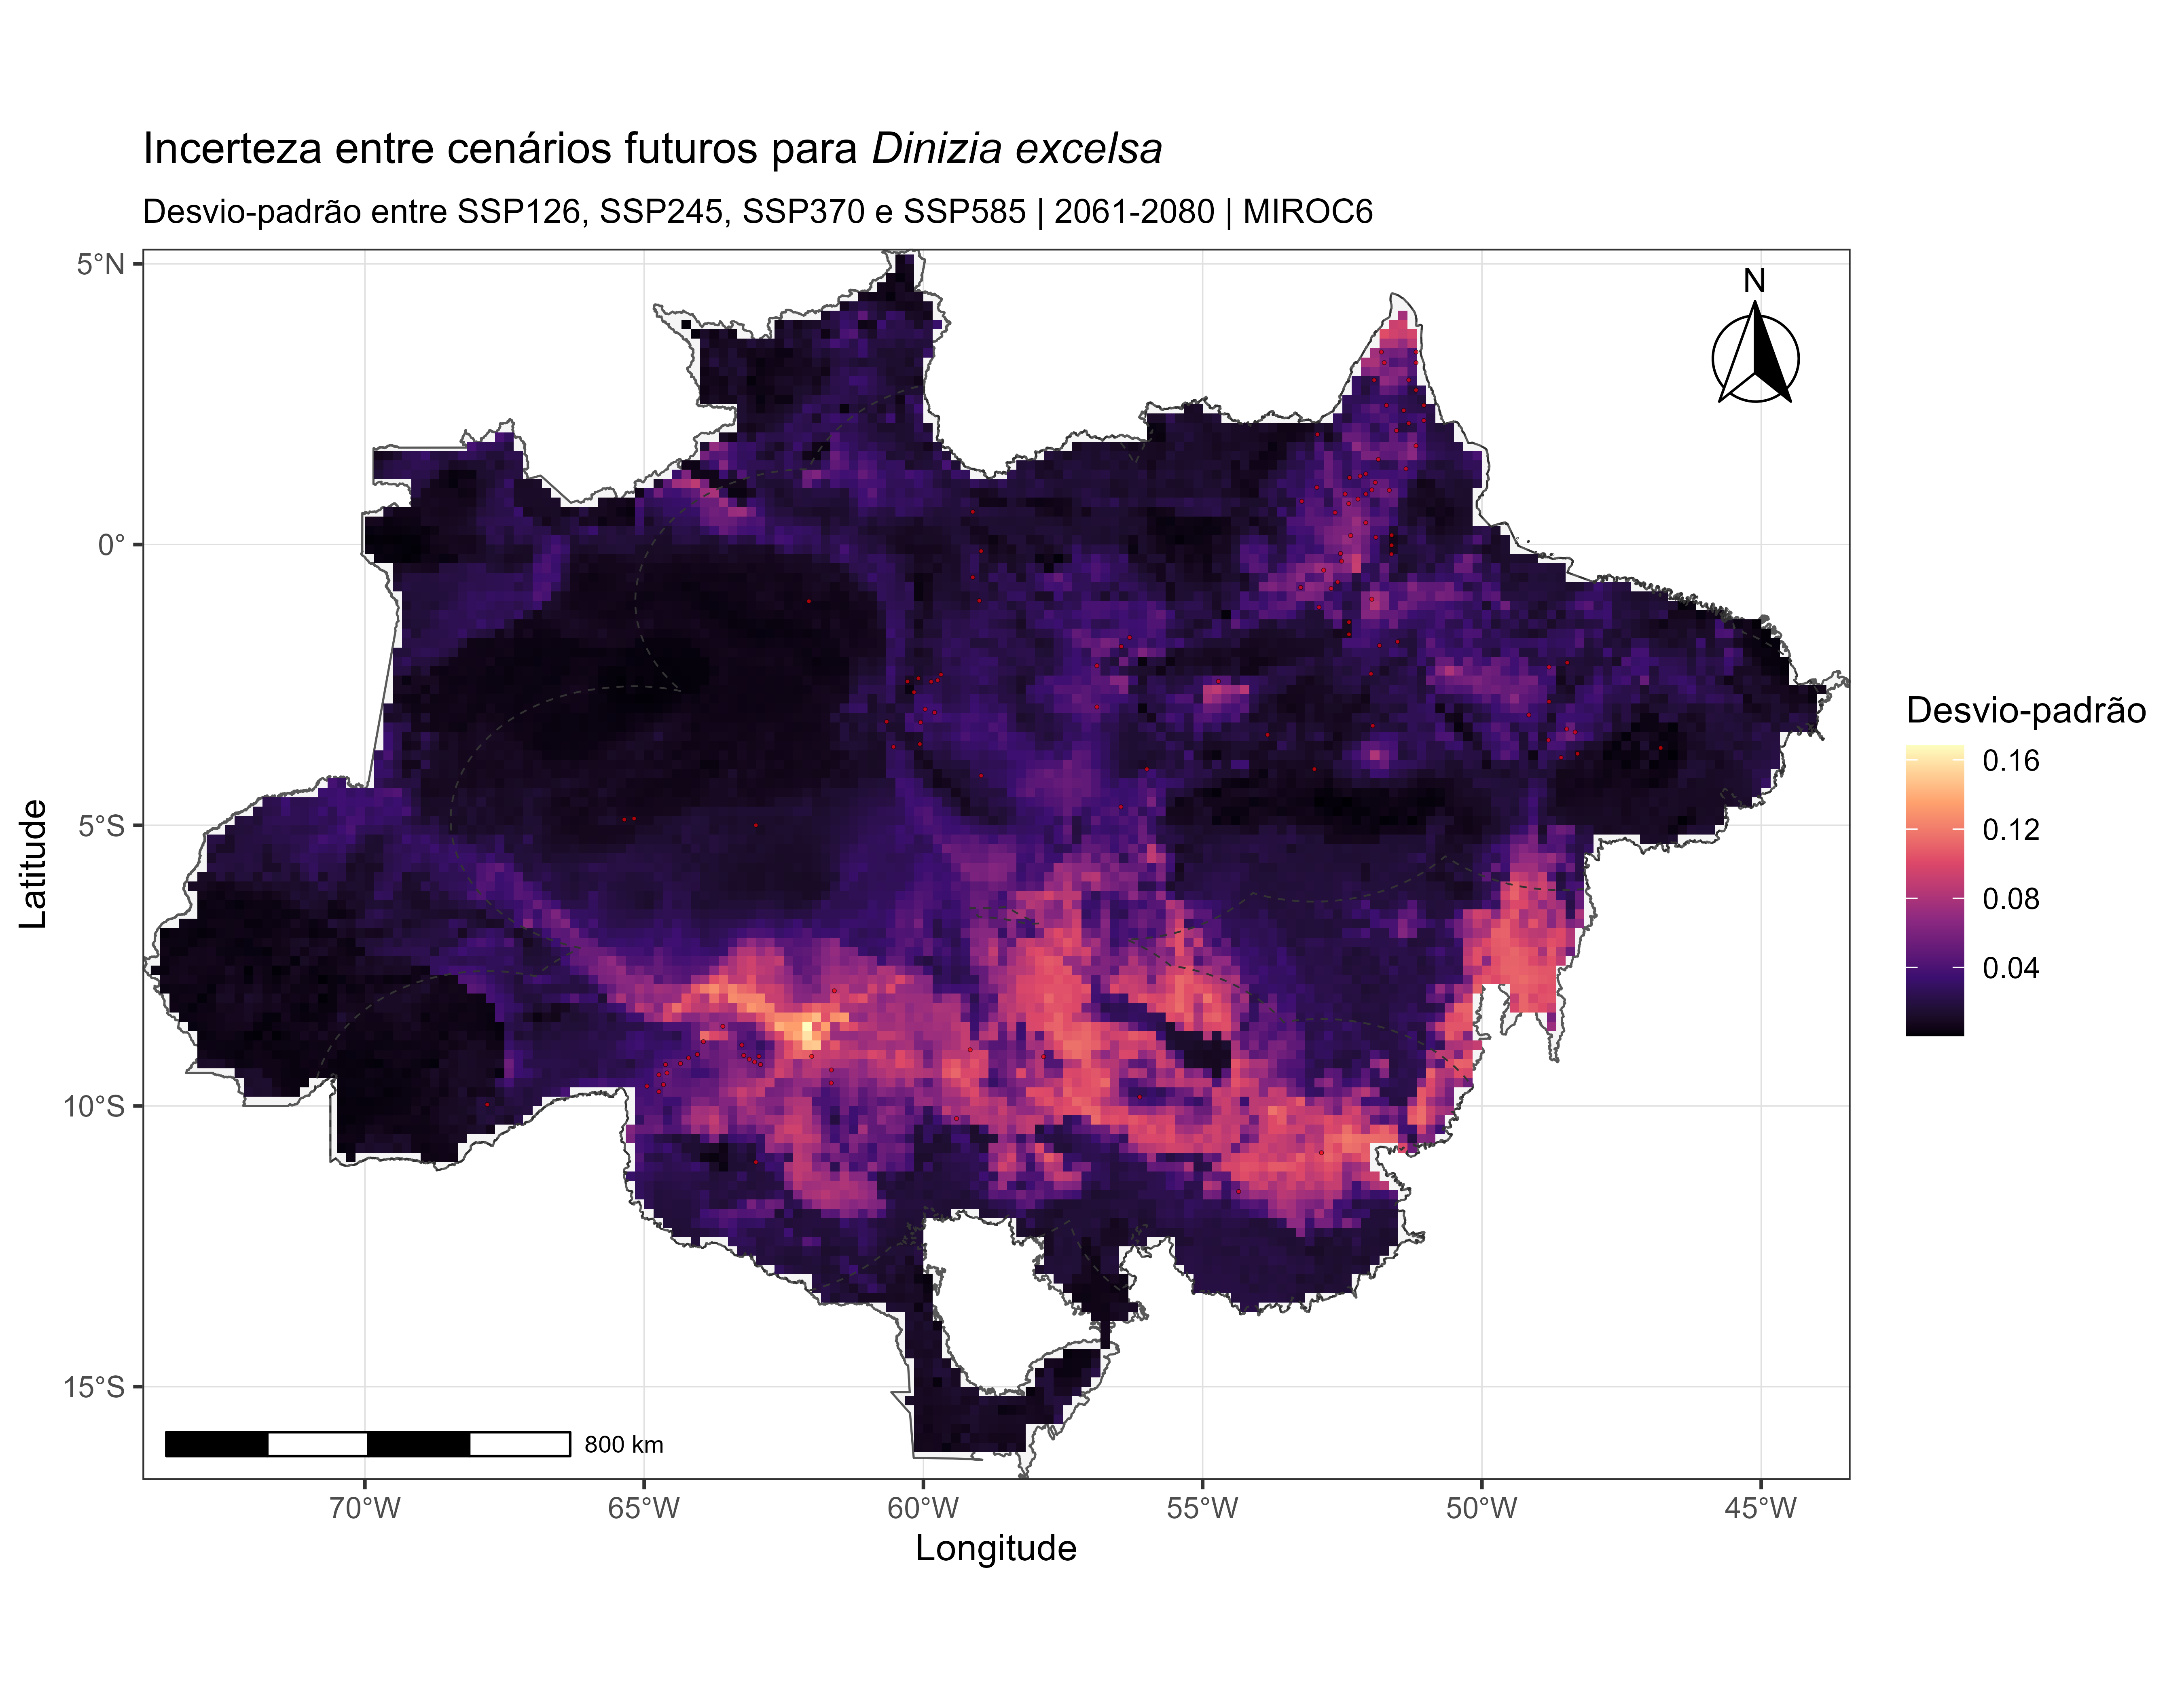
\includegraphics[width=0.88\textwidth]{figuras/unidade16/unidade16_incerteza_cenarios_futuros.png}
	\caption{Incerteza entre cenários futuros para \textit{Dinizia excelsa}, estimada pelo desvio-padrão entre ensembles SSP126, SSP245, SSP370 e SSP585.}
	\label{fig:unidade16_incerteza_cenarios}
\end{figure}

\section{Incerteza por extrapolação ambiental}

Mapas de extrapolação, como MESS e MOP, indicam áreas onde as condições futuras ou passadas estão fora do domínio ambiental de calibração. Essas regiões devem receber maior peso de incerteza interpretativa.

\rscriptfile{scripts/unidade16/04_incerteza_extrapolacao.R}

\begin{figure}[H]
	\centering
	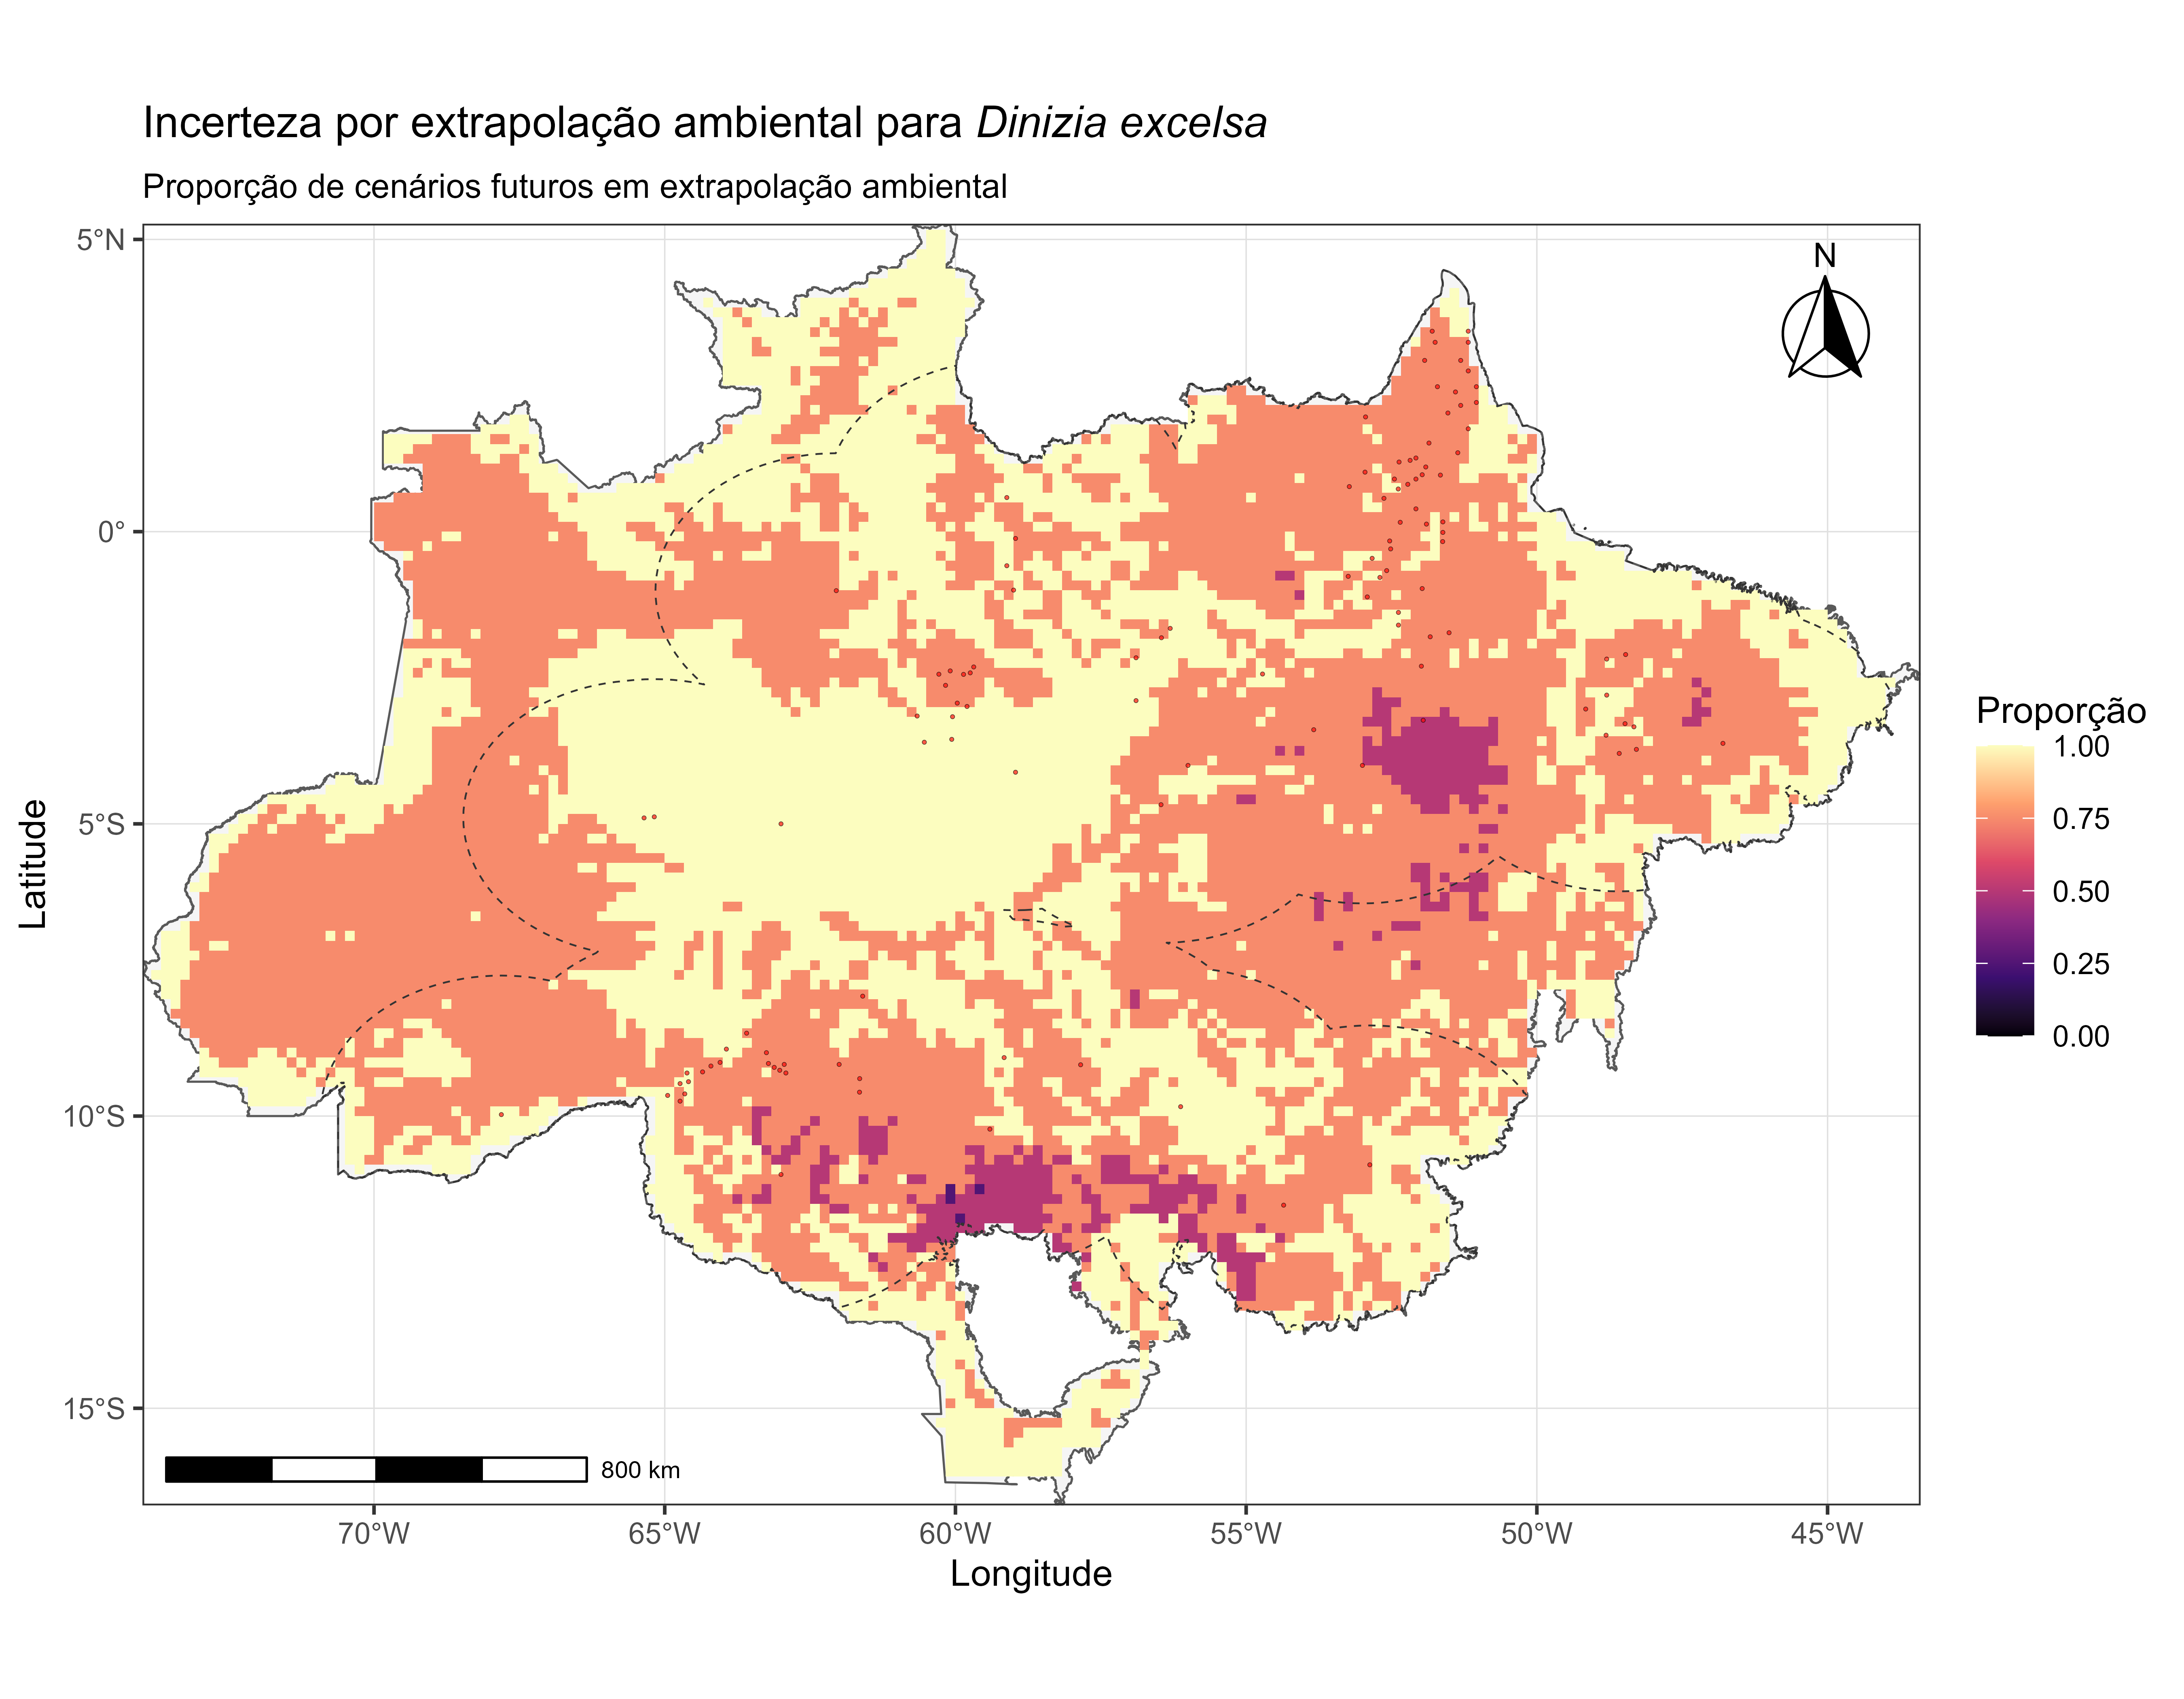
\includegraphics[width=0.96\textwidth]{figuras/unidade16/unidade16_incerteza_extrapolacao.png}
	\caption{Incerteza associada à extrapolação ambiental futura para \textit{Dinizia excelsa}.}
	\label{fig:unidade16_incerteza_extrapolacao}
\end{figure}

\section{Incerteza paleoclimática}

As reconstruções paleoclimáticas possuem incertezas associadas aos modelos climáticos, à resolução espacial, à reconstrução das condições passadas e à hipótese de conservação de nicho. Nesta unidade, avaliamos a variação entre os ensembles paleoclimáticos.

\rscriptfile{scripts/unidade16/05_incerteza_paleoclimatica.R}

\begin{figure}[H]
	\centering
	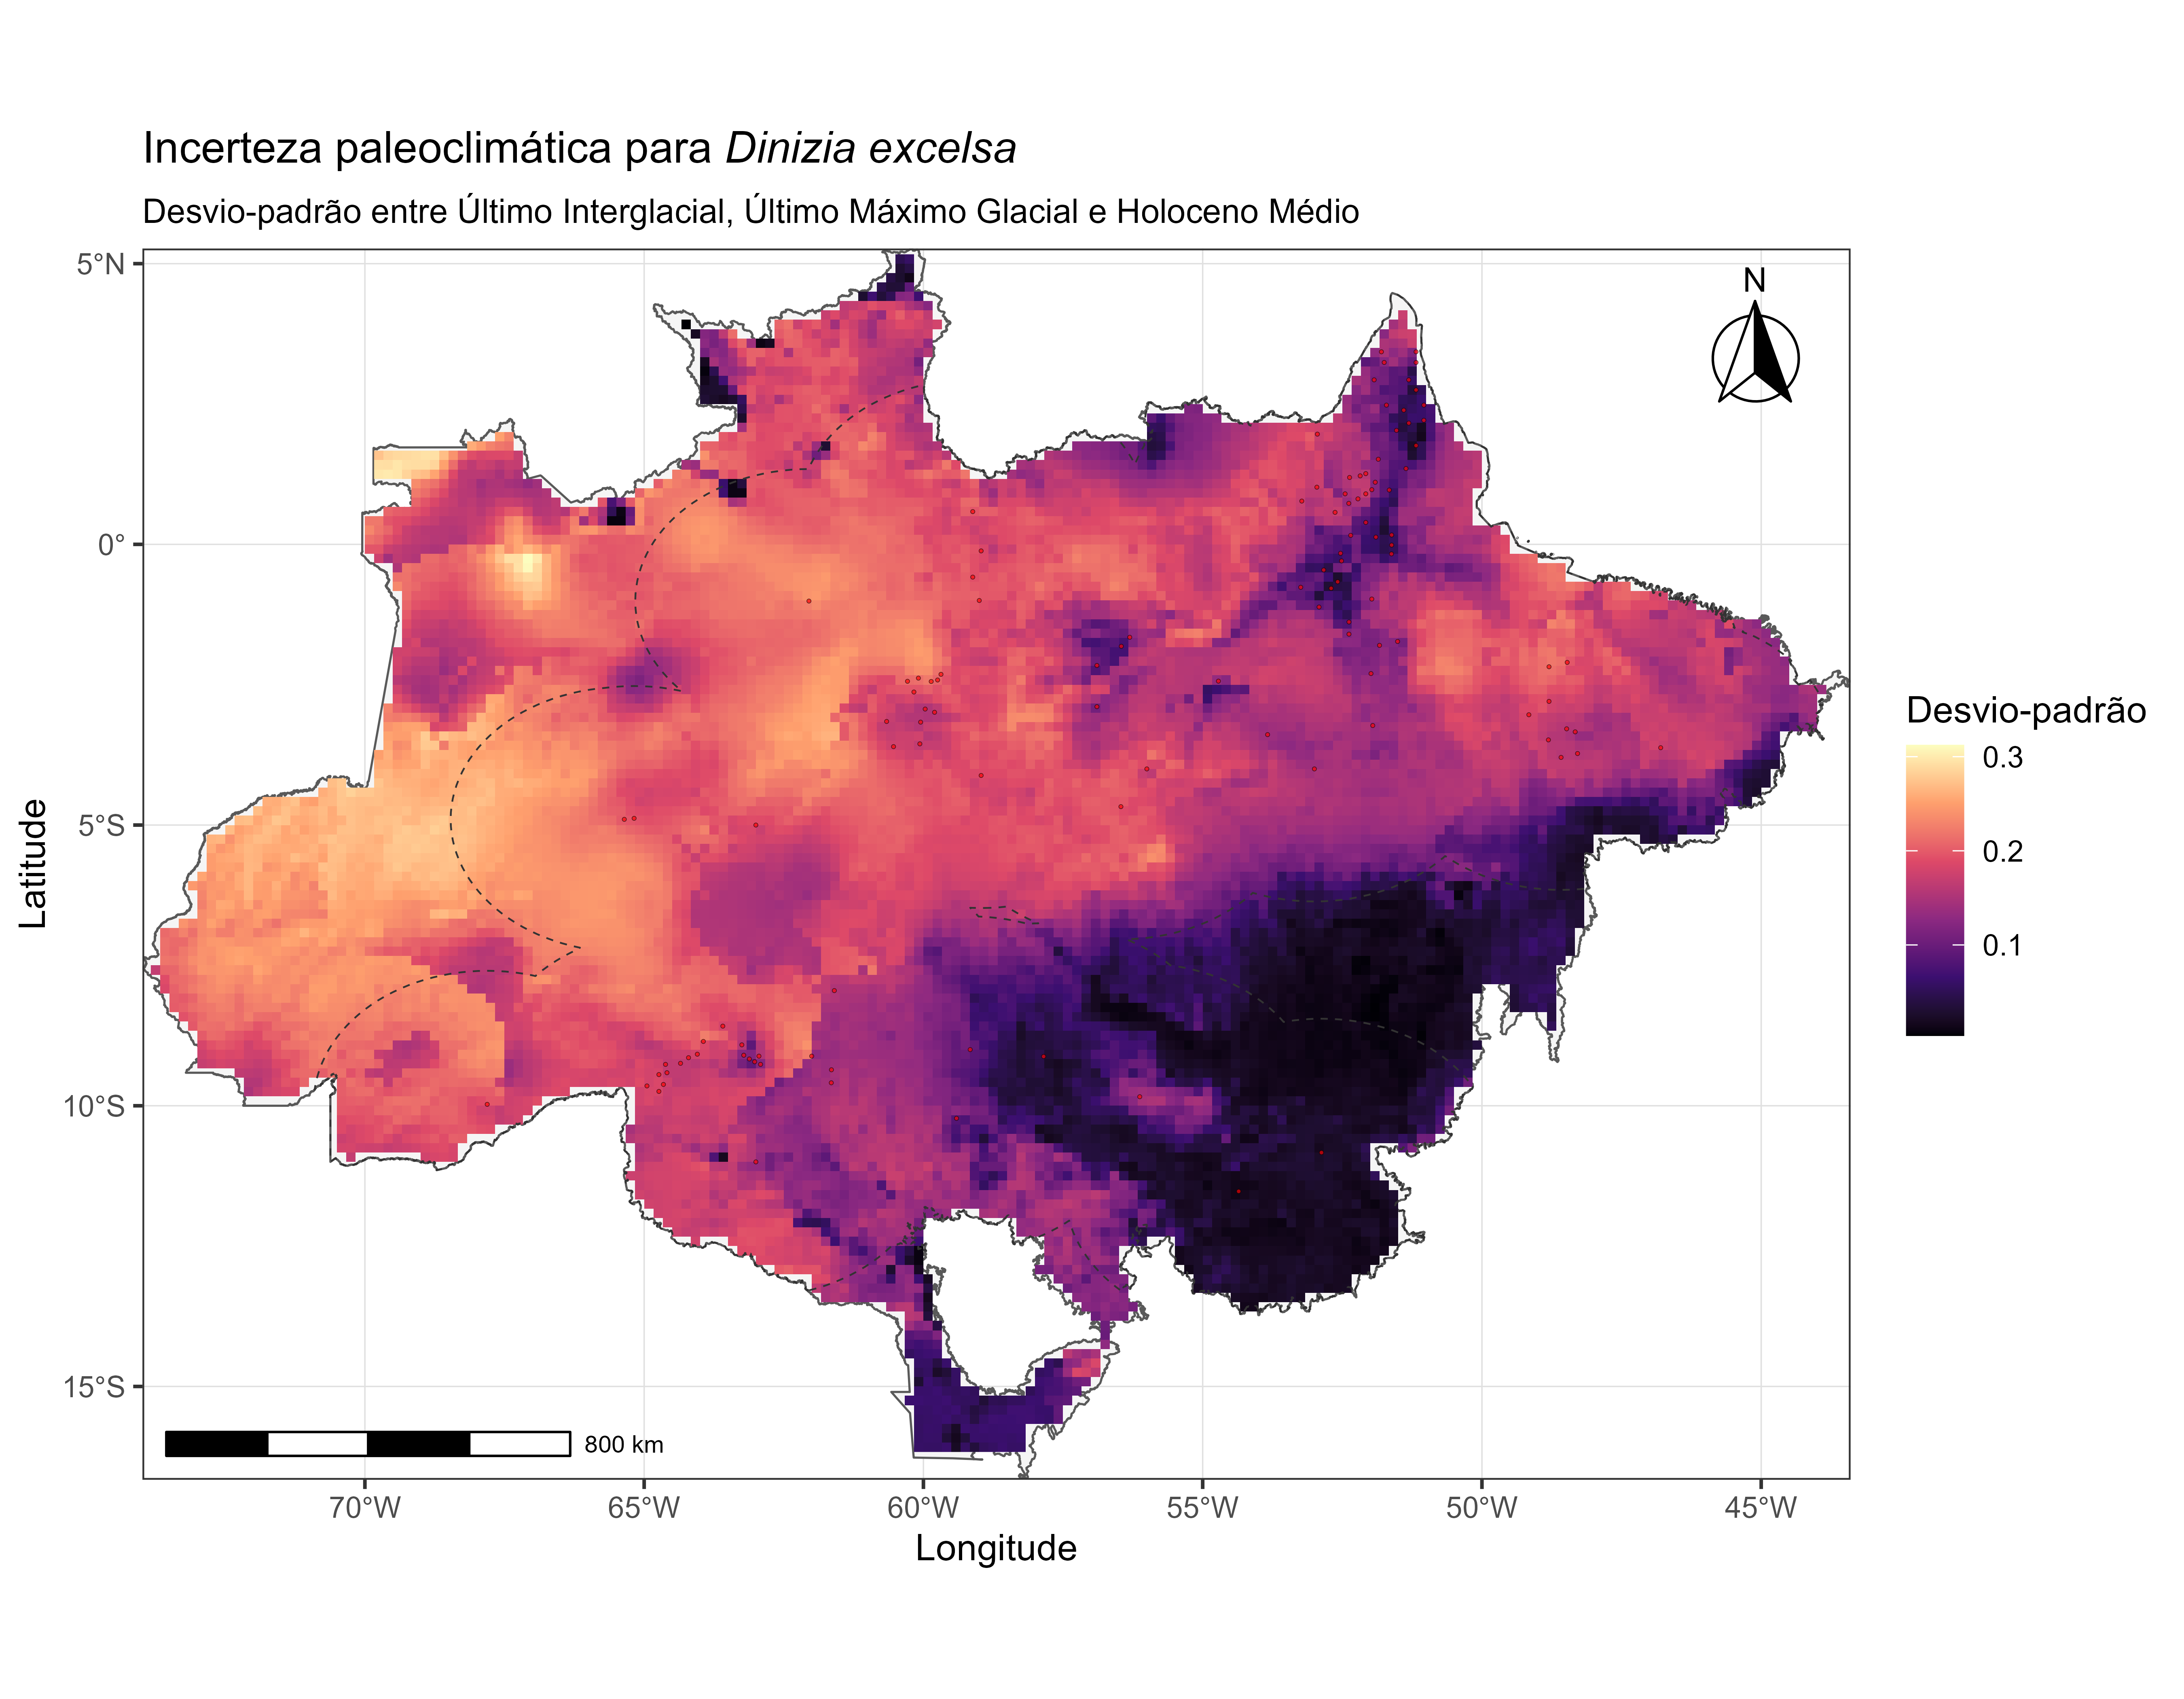
\includegraphics[width=0.88\textwidth]{figuras/unidade16/unidade16_incerteza_paleoclimatica.png}
	\caption{Incerteza paleoclimática estimada pela variação entre períodos passados para \textit{Dinizia excelsa}.}
	\label{fig:unidade16_incerteza_paleo}
\end{figure}

\section{Incerteza integrada}

A incerteza integrada combina diferentes fontes em uma superfície única, permitindo identificar regiões onde as predições são mais robustas e regiões onde a interpretação deve ser mais cautelosa.

\rscriptfile{scripts/unidade16/06_incerteza_integrada.R}

\begin{figure}[H]
	\centering
	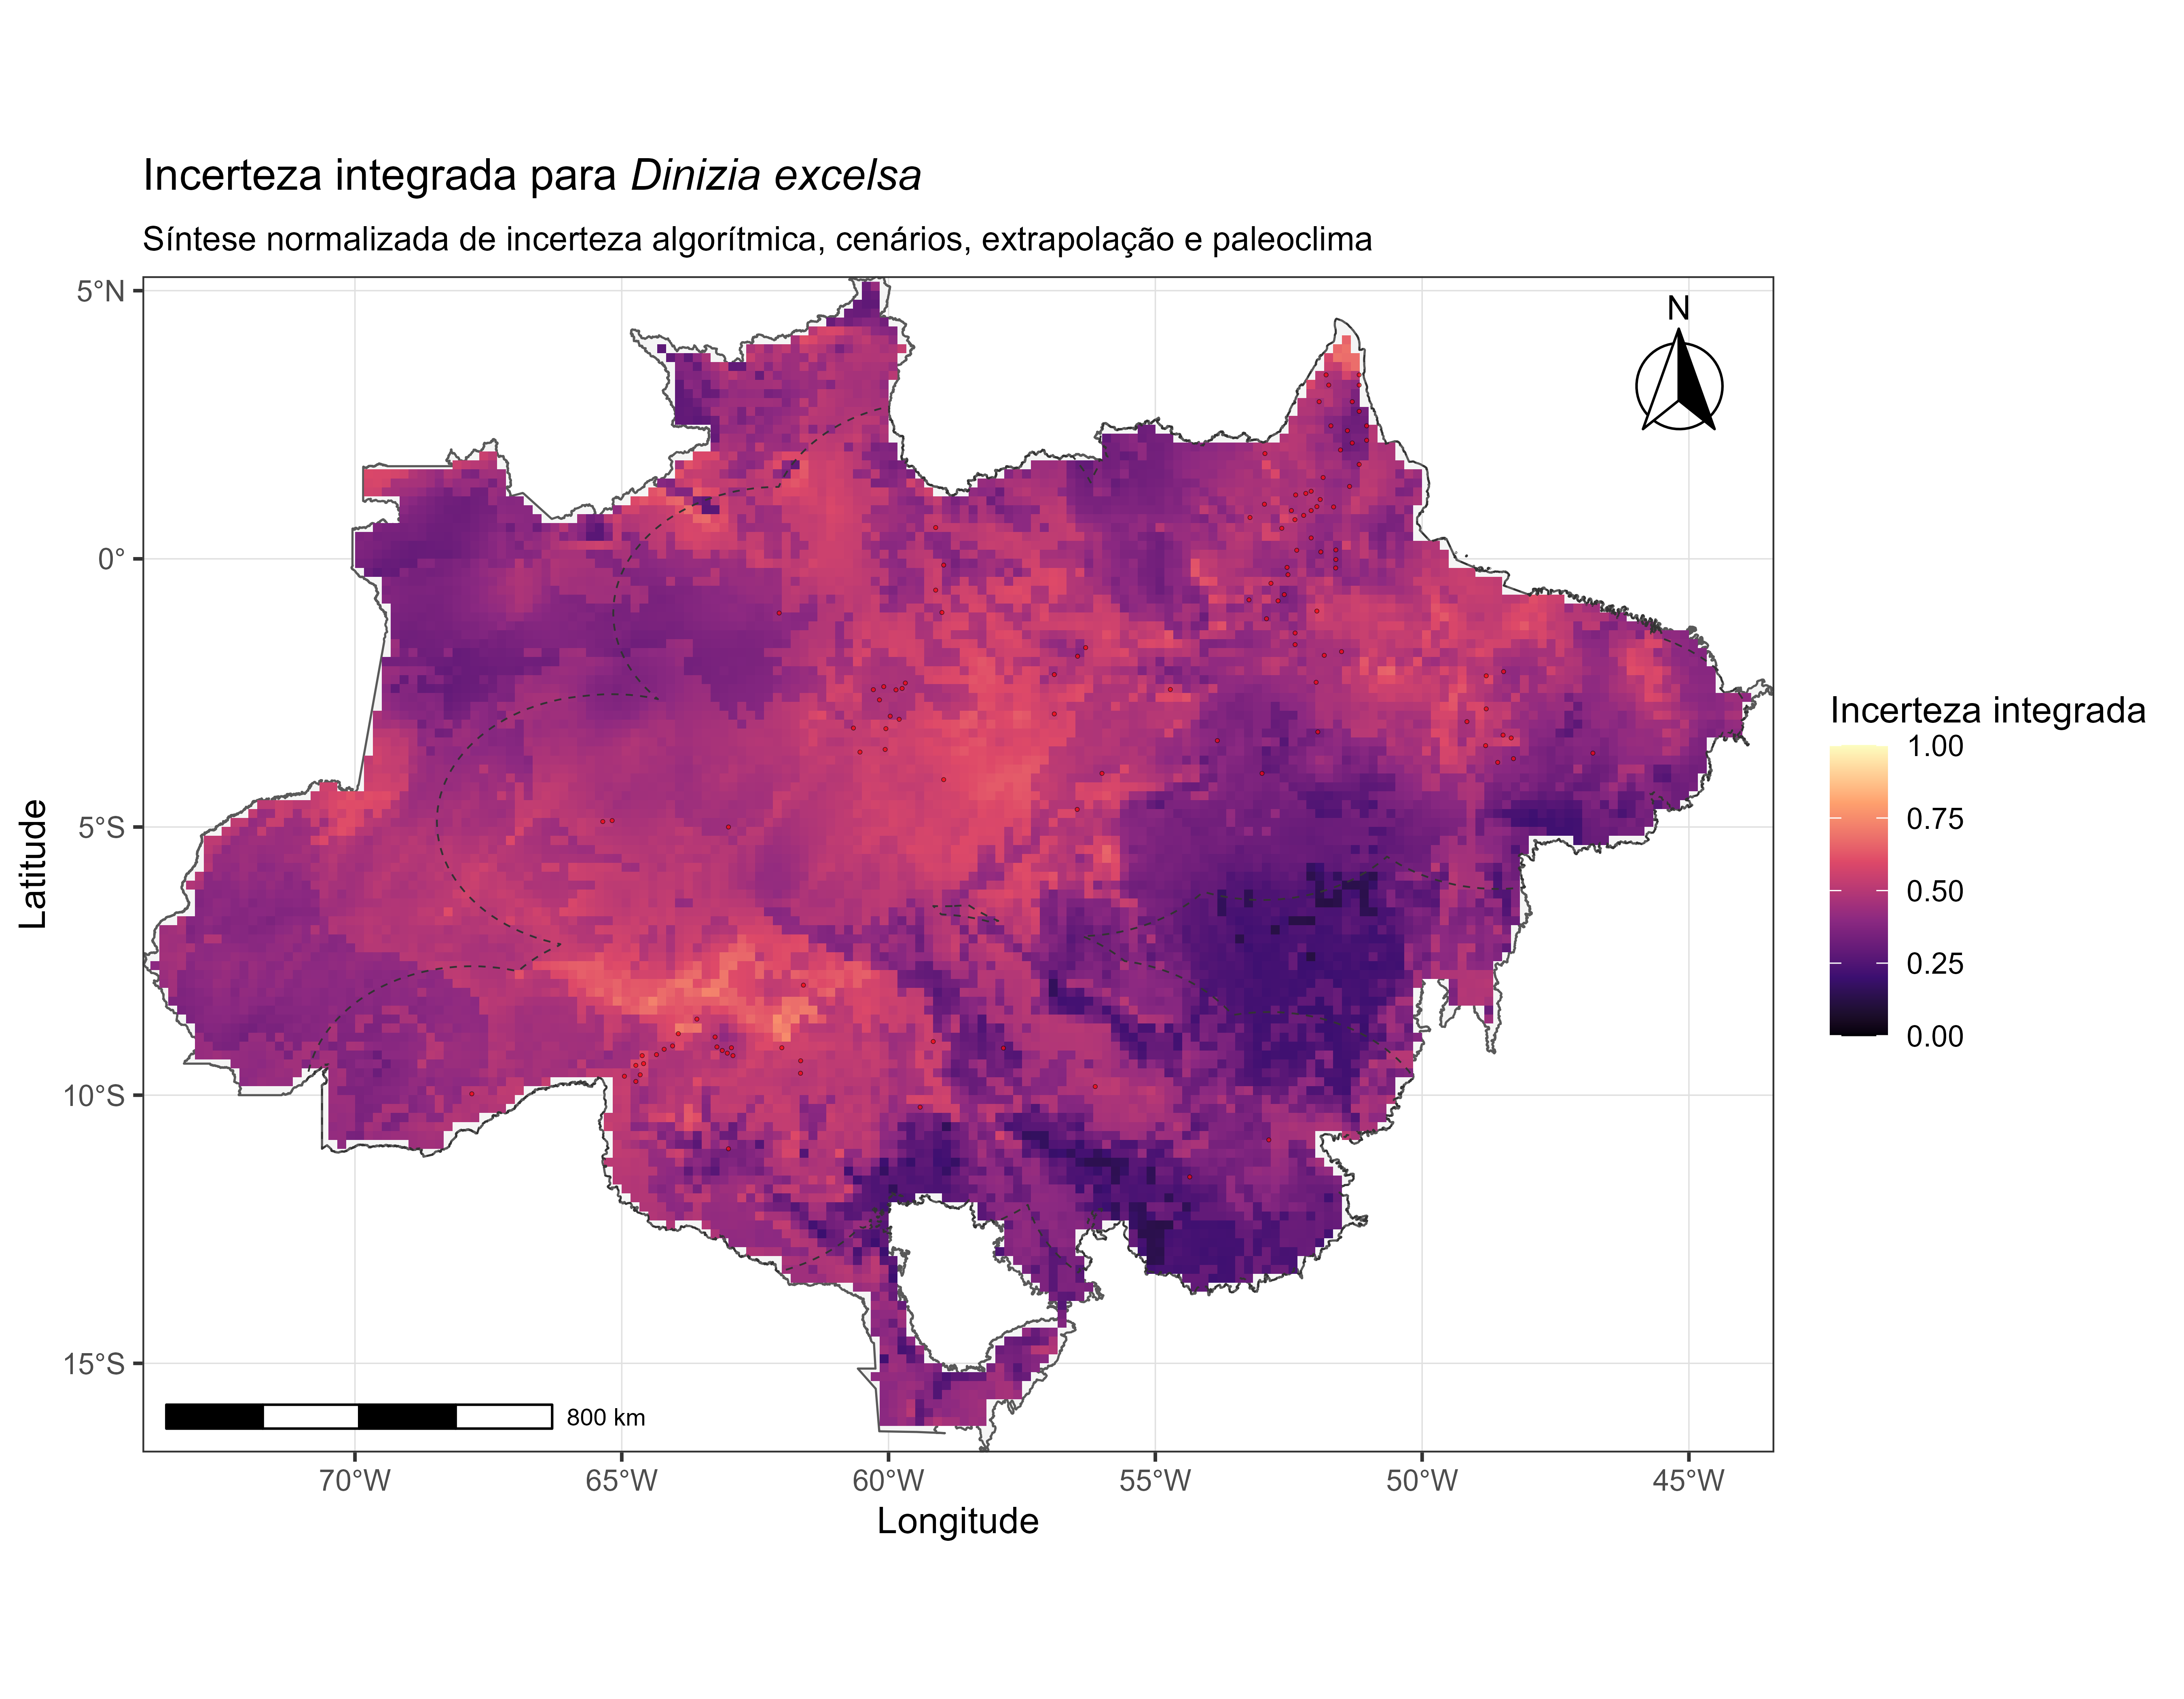
\includegraphics[width=0.88\textwidth]{figuras/unidade16/unidade16_incerteza_integrada.png}
	\caption{Mapa de incerteza integrada para \textit{Dinizia excelsa}, combinando incerteza algorítmica, incerteza entre cenários, extrapolação ambiental e incerteza paleoclimática.}
	\label{fig:unidade16_incerteza_integrada}
\end{figure}

\section{Adequabilidade versus incerteza}

Um resultado útil em conservação é identificar áreas com alta adequabilidade e baixa incerteza. Essas áreas representam regiões mais robustas para interpretação ecológica e priorização espacial.

\rscriptfile{scripts/unidade16/07_adequabilidade_incerteza.R}

\begin{figure}[H]
	\centering
	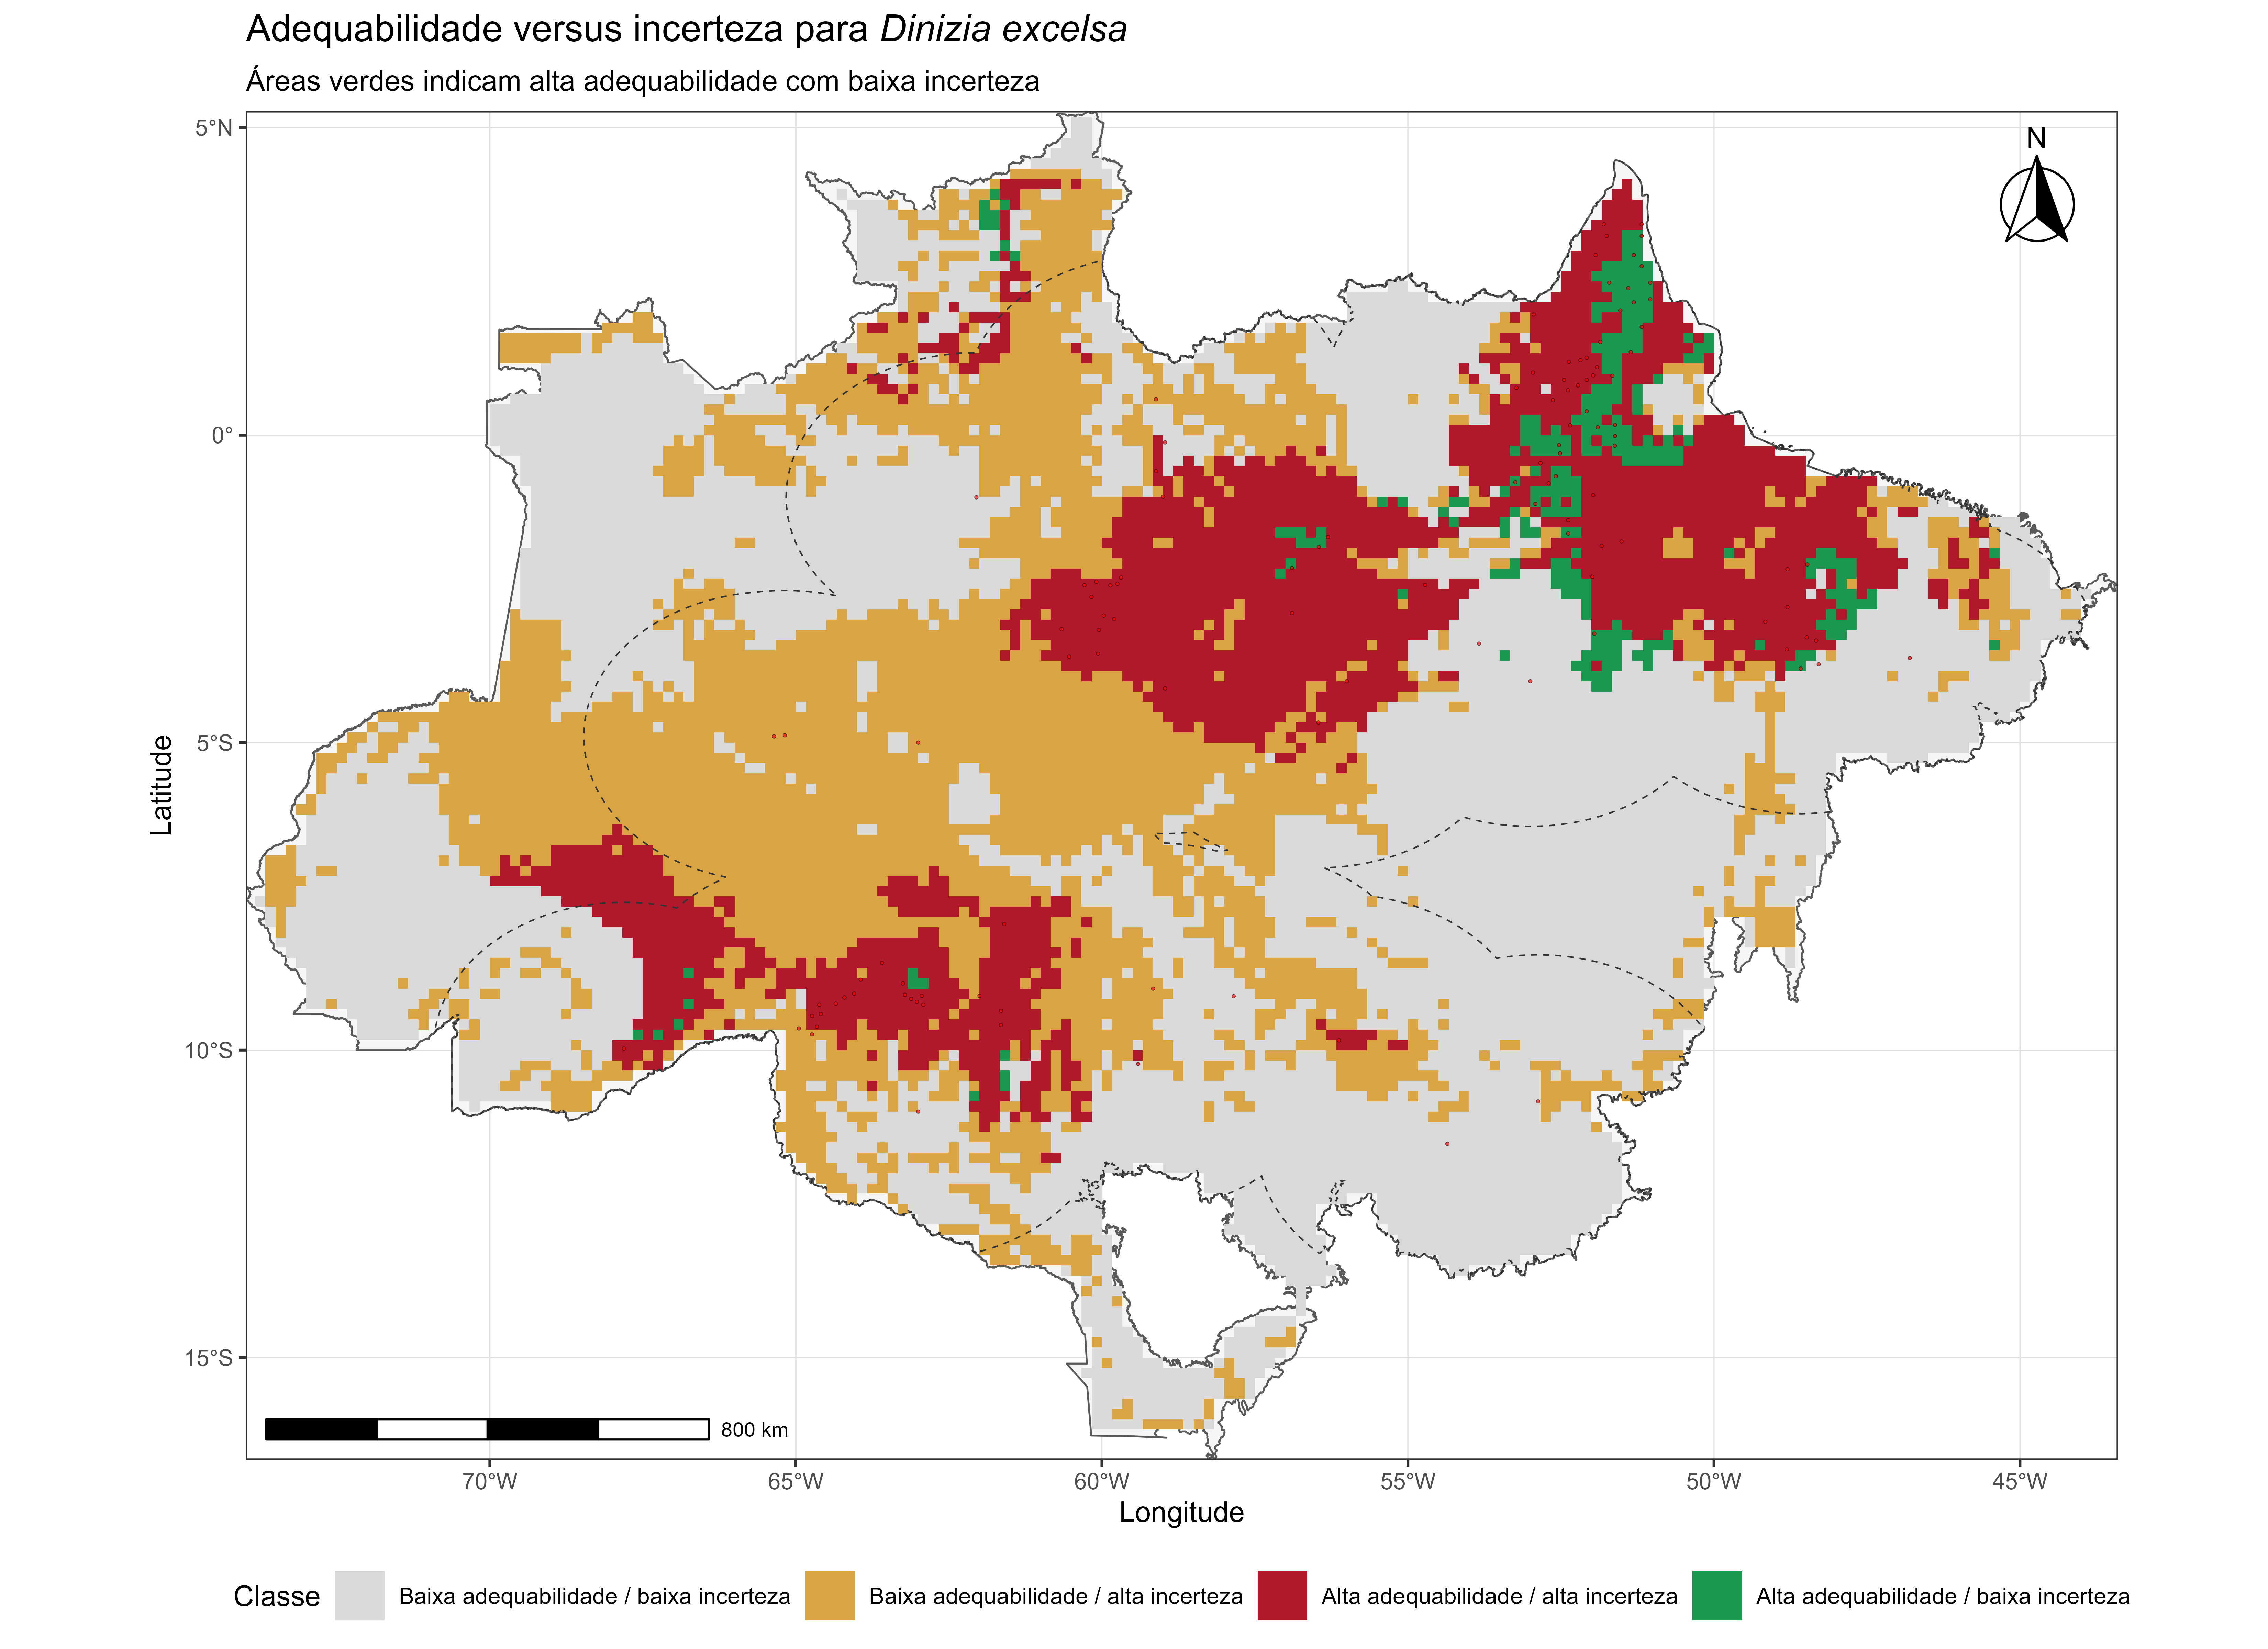
\includegraphics[width=0.96\textwidth]{figuras/unidade16/unidade16_adequabilidade_incerteza.png}
	\caption{Classificação combinada de adequabilidade e incerteza para \textit{Dinizia excelsa}.}
	\label{fig:unidade16_adequabilidade_incerteza}
\end{figure}

\section{Síntese das incertezas}

\rscriptfile{scripts/unidade16/08_sintese_incertezas.R}

\begin{figure}[H]
	\centering
	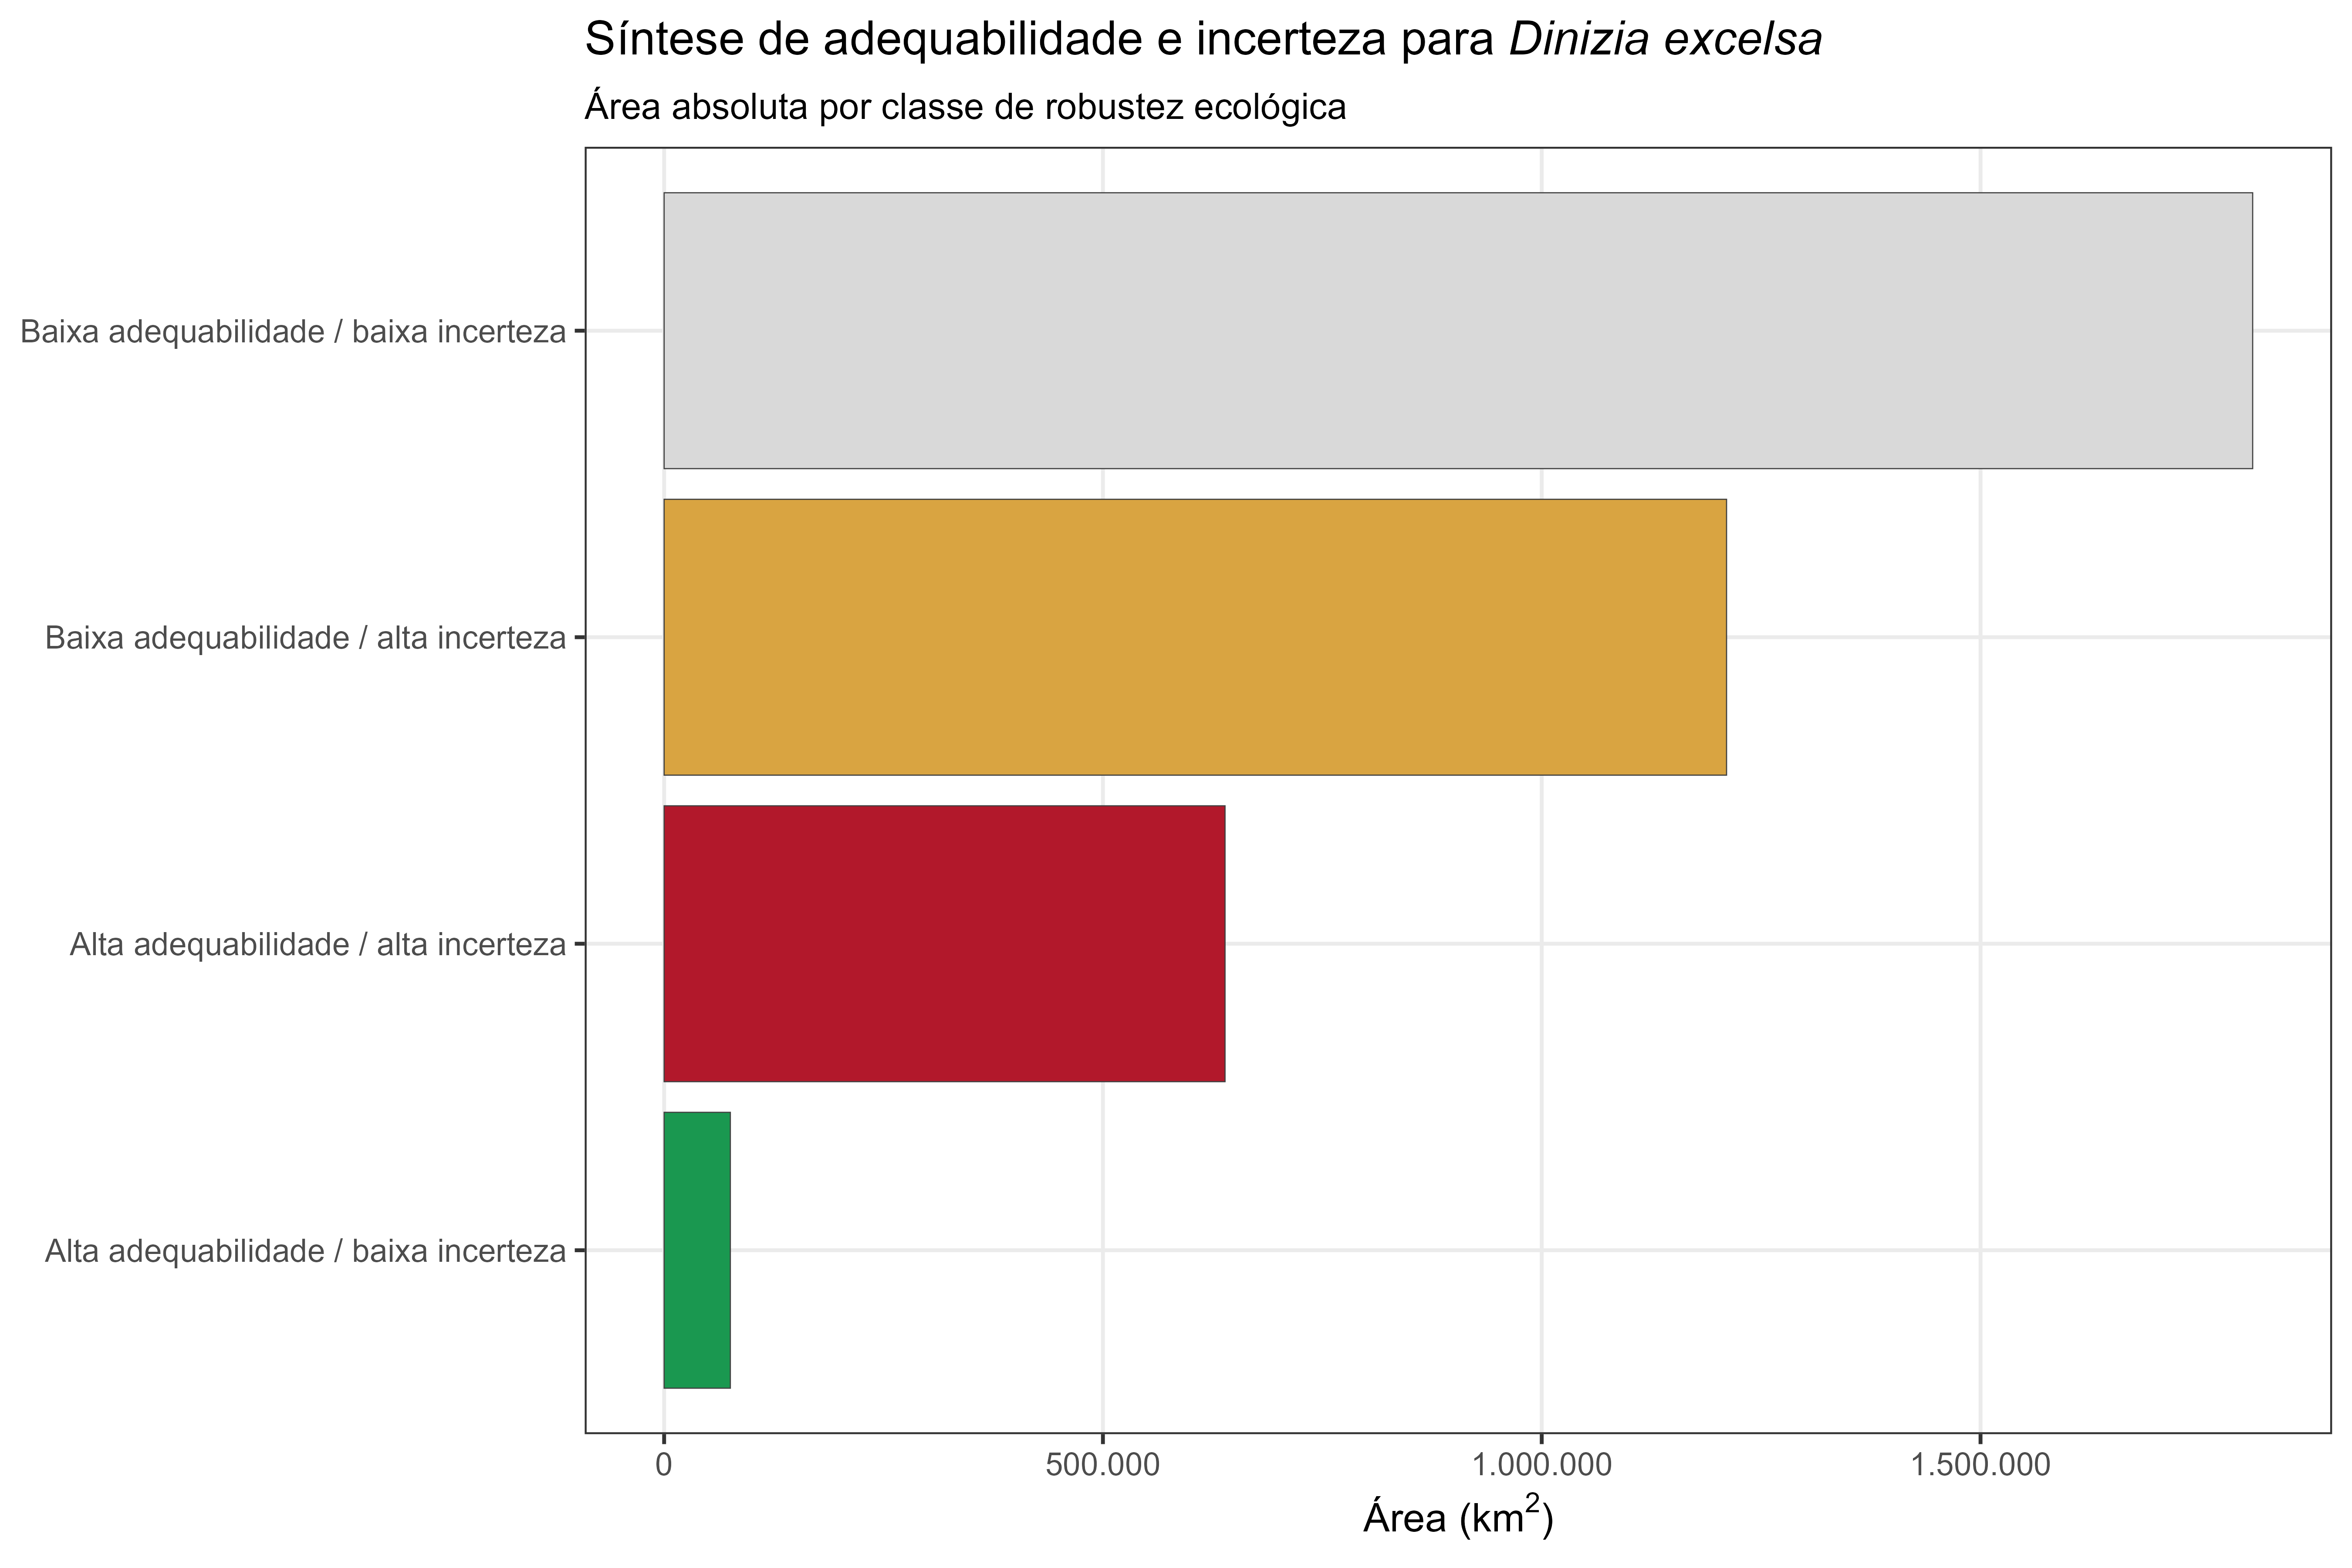
\includegraphics[width=0.88\textwidth]{figuras/unidade16/unidade16_sintese_incertezas.png}
	\caption{Síntese quantitativa das classes de adequabilidade e incerteza para \textit{Dinizia excelsa}.}
	\label{fig:unidade16_sintese}
\end{figure}

\section{Pipeline completo}

\rscriptfile{scripts/unidade16/09_pipeline_incertezas.R}

\section{Síntese da unidade}

A análise de incertezas transforma SDM de um produto cartográfico simples em uma ferramenta científica mais robusta. Para \textit{Dinizia excelsa}, a integração entre incerteza algorítmica, cenários futuros, extrapolação e paleoclima permite distinguir áreas de alta confiança de áreas onde os resultados devem ser tratados como hipóteses.

\begin{conceito}[title={\faBook\quad Mensagem central}]
	A interpretação de SDM deve sempre considerar duas perguntas simultâneas: onde o modelo indica alta adequabilidade e quão confiável é essa estimativa?
\end{conceito}

\section{Exercícios de fixação}

\begin{enumerate}
	\item Liste cinco fontes de incerteza em SDM.
	\item Explique o que é incerteza algorítmica.
	\item Por que cenários SSP diferentes produzem incerteza?
	\item Como MESS e MOP contribuem para interpretar incerteza?
	\item Por que projeções paleoclimáticas possuem incerteza própria?
	\item Como interpretar uma área com alta adequabilidade e alta incerteza?
	\item Como mapas de incerteza podem apoiar decisões de conservação?
\end{enumerate}

% ============================================================
% UNIDADE 17
% ============================================================

